\chapter*{\FontH{\Huge Die Papageieninsel}}
\addcontentsline{toc}{chapter}{Die Papageieninsel}
\lettrine[lines=3]{\color{DeepPink}N}{och} bevor die Sonne aufgegangen war, wurde Winnimon vom Smutje geweckt. Winnimon war der Schiffsjunge der Drachenblume, einem Piratenschiff, das alle sieben Meere befuhr. Natürlich wehte auf dem Schiff, die Jolly Roger, die berühmte Piratenfahne, aber das war mehr zur Abschreckung. So richtige Piraten waren sie nicht hier auf der Drachenblume. Schatzsucher wäre wohl die bessre Berufsbezeichnung gewesen, aber da durfte man nicht kleinlig sein. Die Piraten waren sehr schnell beleidigt.

Bisher hatte Winnimon nur langweilige Aufgaben erledigen dürfen: das Deck schrubben, Kartoffeln schälen und die Regenwürmer füttern, die zum Angeln benötigt wurden, falls der Smutje Fisch kochen wollte. Der Smutje ist der Koch auf einem Schiff und war ein guter Freund von Winnimon, aber eben auch sein Chef. Schon lange hatte er ihm versprochen, auch einmal etwas Spannendes machen zu dürfen. Und da der Kapitän in der Nacht zuvor seinen 53-ein-Drittelsten Geburtstag gefeiert hatte, waren die anderen Piraten nicht so Recht in der Lage, auf Schatzsuche zu gehen. Da musste eben Winnimon ran, denn der war noch zu jung und daher zu vernünftig Geburtstage so zu feiern, wie das erwachsene Piraten machen.

Die Schatzsuche, von der die Piraten lebten, war eine eher leichte Aufgabe. Jedenfalls viel weniger anstrengend, als andere Schiffe zu überfallen, wie das Piraten normalerweise machen. Erst muss man herausbekommen, wo ein Schatz zu finden ist, dann dort hin segeln, dann ausgraben, fertig. Schwierig war daran nichts, ausser dass man genügend gültige Schatzkarten vorrätig haben musste, aber das war auf der Drachenblume kein Problem, der Kapitän hatte die geerbt. Segeln machte sowieso allen Spass. Das Mühsamste an der ganzen Aufgabe war daher den Schatz zu bergen, aber da Schätze meist auf einsamen Inseln wohnen, genügte es, wenn jeweils einer der Piraten los zog und die Arbeit erledigte.

Eigentlich war der Smutje jetzt an der Reihe aber der hatte noch so fürchterliche Kopfschmerzen von letzter Nacht, dass er lieber Winnimon los schickte, als selber zu gehen.

\begin{center}
{ $\skull$}
\end{center}

\enquote{Winnimon, aufwachen. Du gehst heute auf Schatzsuche.} Winnimon war wie elektrisiert. Noch ehe der Smutje sich einmal richtig umgedreht hatte, war Winnimon aus seiner Koje gesprungen und stand angezogen da. Auf so einen Auftrag hatte er sich schon lange gefreut!

\enquote{Leise, die anderen schlafen noch. Hier ist ein Sack mit deinem Proviant. Du nimmst jetzt das Beiboot und ruderst zu der kleinen Insel da vorne. Auf der Insel ist ein Berg und in dem Berg eine Höhle und in der Höhle der Schatz. Du gehst voraus und suchst den Schatz, wir anderen kommen später hinterher und helfen dir beim Transport. Das ist auch nicht weiter gefährlich, die Insel ist unbewohnt, so steht es hier auf der Karte.}

So ruderte Winnimon durch die Dunkelheit, immer ein Schlag nach dem anderen. Nur gut, dass Vollmond war. Nach einer Stunde war er bei der Insel, die Sonne war mittlerweile auch aufgegangen und wärmte schon recht angenehm. Also nochmals schnell ins Meer gesprungen, denn der Weg zu dem Berg sah lang aus und hoch war der auch. Ausserdem war die Insel stark bewaldet und Winnimon war erfahren genug, um zu wissen, dass man sich in einem so dichten Wald nur orientieren kann, wenn man ungefähr ahnt, wo die Sonne steht. Und das klappt erst, wenn sie hoch genug steht und das tat sie noch nicht.

Also rein ins Wasser und ein wenig von den Wellen treiben lassen. Gerade als Winnimon wieder mit dem Kopf aus dem Wasser guckte hörte er eine krächzende Stimme.

\enquote{Besuch, Besuch, Besuch, wir haben Besuch.}, und sofort wiederholte ein grosser Chor von genauso krächzenden Stimmen, \enquote{Besuch, Besuch, Besuch, Besuch.}

Winnimon verhielt sich ganz still und sah sich um. Kein Mensch war zu sehen, lediglich ein paar bunte Vögel sassen auf den Bäumen. Wo hatten sich wohl die vielen Menschen versteckt, die da gerade noch gerufen hatten? Vorsichtig kam Winnimon aus dem Wasser und schlüpfte in seine Kleider. Nicht vorzustellen, dass er nackt war, wenn hier gleich ein paar Dutzend Leute angelaufen kamen.

\enquote{Was will er wohl? Was will er wohl?}, hörte er die Stimmen wieder. Aber sehen konnte er noch immer niemanden. Der Wald, der gleich hinter dem Strand begann, war dicht, da konnte man sich gut verstecken. Er nahm seinen Mut zusammen und rief laut: \enquote{Ich bin Winnimon, Pirat auf der Drachenblume. Wer seid ihr? Zeigt euch ihr Feiglinge!}

Und der Chor antwortete: \enquote{Er sieht uns nicht, er sieht uns nicht.}

\afterpage{
    \begin{figure}
        \thispagestyle{empty}
        \centering
        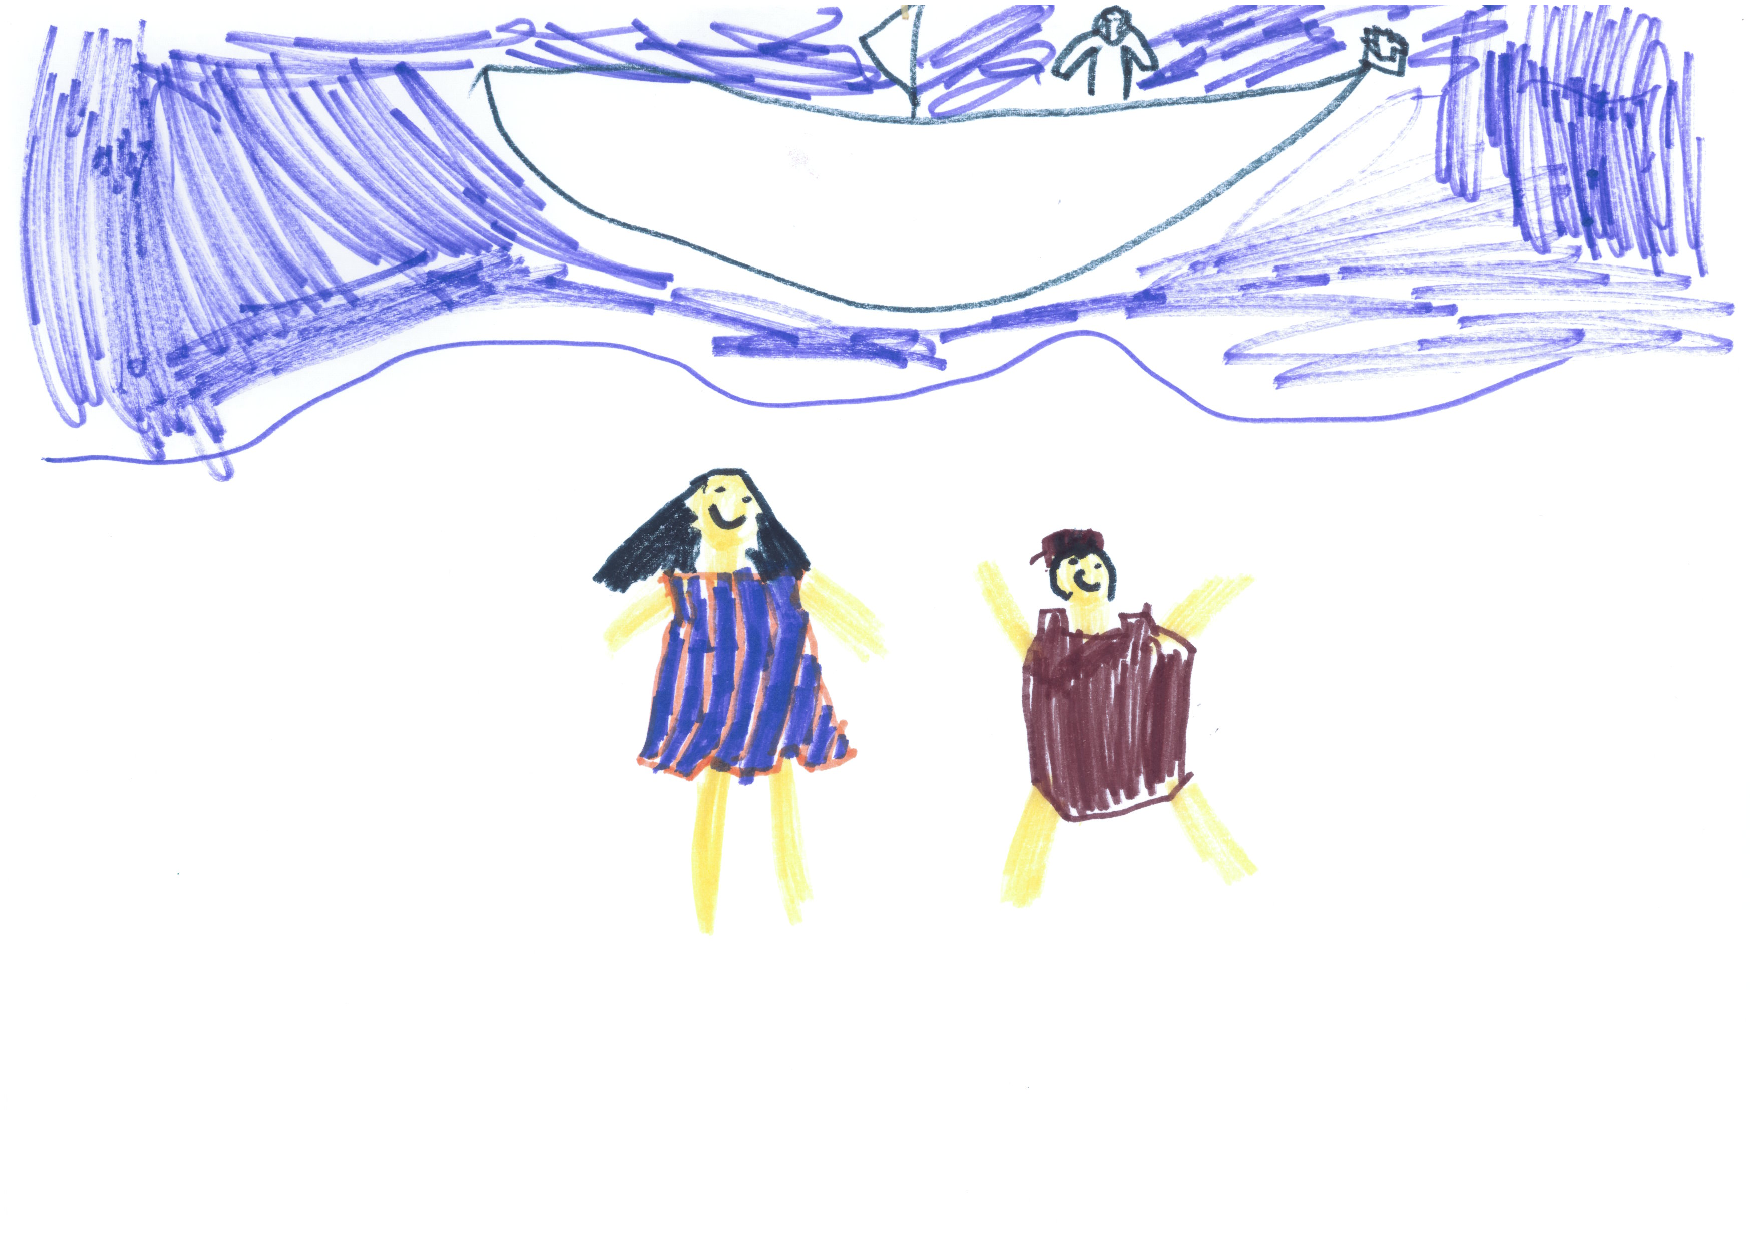
\includegraphics[width=\textwidth]{bilder/pirat1.pdf}
    \end{figure}
    \clearpage
}


Da begriff Winnimon, wer da gerufen hatte. Die Papageien! Natürlich, davon hatte er gehört, dass Papageien sprechen können. Aber sicher war er sich nicht. Das beste wäre es wohl gewesen zu warten, bis die anderen Piraten vom Schiff kamen, dann könnte man gemeinsam nachsehen. Aber das wäre natürlich sehr peinlich gewesen. Die anderen Piraten hätten Winnimon wochenlang geärgert, wenn er vor ein paar Papageien Angst gehabt hätte. 

Da kam ihm eine Idee. Er öffnete den Sack mit dem Brot, den er vom Smutje bekommen hatte, brach etwas Brot ab und verstreute es am Strand. Dann setzte er sich daneben und wartete. Es dauerte auch nicht lange, da kamen die ersten Papageien angeflogen. Herrlich bunt glitzerten ihre Federn in der Morgensonne.

Der erste mutige Papagei landete ganz in seiner Nähe. Er neigte den Kopf zur Seite und kam langsam immer näher gehüpft. Er schnappte sich ein Stück vom Brot und sprang wieder zurück. Von dem Beispiel ermutigt kamen noch mehr Papageien und knabberten Brot. 

\enquote{Ich bin hier, weil ich einen Schatz suche}, begann Winnimon zu sprechen, als er merkte, dass sich die Papageien hier sicher fühlten.

\enquote{Einen Schatz sucht er, einen Schatz.} Winnimon begann es etwas zu nerven, dass die Papageien immer alles doppelt sagen mussten.

\enquote{Aber wir verraten nicht, wo die leckersten Früchte wachsen, verraten wir nicht.} Winnimon musste lachen. Papageien halten natürlich ganz andere Dinge für einen Schatz als Menschen.

\enquote{Nein, ich will euch nicht eure Früchte wegnehmen. Ich suche einen Schatz aus Gold und Edelsteinen. Er muss in einer Höhle in einem Berg hier auf eurer Insel sein.}

\begin{center}
{ $\skull$}
\end{center}

Nachdem Winnimon versprechen musste, dass er tatsächlich keine Früchte wollte, willigten die Papageien ein, ihm den Weg zu zeigen. Das war erst etwas mühsam, denn wenn Papageien etwas versprechen, rupfen sie sich dazu eine Feder aus, als Zeichen, dass sie es wirklich ernst meinen. Federn wuchsen aber Winnimon genau so viele wie anderen Menschen auch, nämlich keine. Der Vorschlag, ersatzweise ein Haar zu geben, wurde von den Papageien abgelehnt, denn die Haare der Menschen und das Fell bei Tieren gilt unter allen Vögeln als furchtbar hässlich, womit sie wohl auch Recht haben, wenn man bedenkt, wie schön doch Federn sein können. Zum Glück fanden sie aber die letzten Reste aus dem Essenssack ebenso überzeugend wie eine Feder. 

Die Papageien flogen also voraus und Winnimon lief hinterher. Erst fand er es lustig, dass die Papageien ein Lied nach dem anderen zu singen wussten, aber irgendwann bekam er von den krächzenden Stimmen Kopfschmerzen. Es wäre natürlich sehr unhöflich gewesen, die Vögel zu bitten aufzuhören. 

Die Papageien kennengelernt zu haben, stellte sich für Winnimon als praktisch heraus. Er hatte zwar jetzt selbst nichts mehr zum Essen und ihm knurrte der Magen, dafür wäre er aber ohne die Papageien viel weniger schnell durch den Wald gekommen. Die kannten sich hier einfach besser aus. Und wenn selbst sie nicht mehr weiter wussten, brauchten sie nur über die Baumwipfel zu fliegen und konnten nachsehen, in welche Richtung der Berg lag.

Gegen Mittag erreichten sie den Fuss des Berges. Die Papageien begleiteten ihn noch ein Stück, meinten aber, dass Papageien niemals auf Berge fliegen würden und dass er ab hier alleine weiter müsse. Papageien gehören in den Urwald, da wo die bunten Blüten sind und die Schmetterlinge fliegen. Triste Berge aus Stein und Geröll seien unter ihrer Würde, belehrten sie Winnimon.

Aber er müsse immer nur in Richtung Bergspitze weiter, dann käme er an die Höhle in der der Schatz sein müsse, sie hätten das jedenfalls so von den Adlern gehört, die hier lebten. Verachtung lag in den Stimmen der Papageien, wenn sie von den Adlern sprachen, was daran lag, dass deren Federn nur braun und weiss seien, sie also eher zu den hässlichen Vögeln gehörten. Papageien sind sehr eitel, merkte Winnimon. Zum Abschied bekam er noch eine besonders schöne rote Feder geschenkt, die er sich an den Hut stecken konnte. 

\enquote{Für den Fall, dass du Mal wieder etwas versprechen musst, versprechen musst.} erklärten sie und verabschiedeten sich von ihm.

\begin{center}
{ $\skull$}
\end{center}

Der Aufstieg war zwar anstrengend, machte aber vor allem auch Spass. Winnimon kletterte nämlich sehr gerne. So dauerte es auch nicht lange, bis er tatsächlich den Eingang einer Höhle gefunden hatte. In der Ferne konnte Winnimon sein Schiff die Drachenblume sehen. Die ersten Boote der anderen Piraten waren bereits unterwegs zur Insel.

Winnimon ging in die Höhle und wartete, bis sich seine Augen an die Dunkelheit gewöhnt hatten. Überall hingen Spinnweben an den Wänden und an der Decke schliefen Fledermäuse, den Kopf nach unten, wie die das so machen. Tagsüber schlafen und nur nachts wach zu sein, wäre nichts für mich, dachte Winnimon. Ein bisschen unheimlich war ihm jetzt schon zu Mute. Eigentlich hatte er keine Angst vor Spinnen, aber diese Spinnweben hier waren \emph{sehr} gross und \emph{sehr} dick. Aber als Pirat hat man keine Angst zu haben, das gehört zur Berufsehre dazu. Also ging Winnimon immer tiefer und tiefer in die Höhle, bis er plötzlich ganz zweifelsfrei ein Schnarchen hörte. Noch jemand, der am Tag schläft.

Winnimon hielt die Luft an, um sich bloss nicht durch das kleinste Geräusch zu verraten. Langsam ging er weiter nach vorne. Er musste erst ein grosses Spinnennetz, das vom Boden bis zur Decke der Höhle reichte, kaputt machen, um zu erkennen, wer da so schnarchte. Zwei Dinge konnte Winnimon im Halbdunkel erkennen: die Schatztruhe, aber leider auch einen riesigen Höhlenbär, der es sich ausgerechnet auf der Truhe gemütlich gemacht hatte.

Und dann noch etwas drittes. Die Spinne, deren Netz er gerade kaputt gemacht hatte, sass auf seinem Arm und krabbelte an ihm hoch. Das Tier war mindestens so gross wie die Hand des Smutje und sie hatte Haare am ganzen Körper. Winnimon musste allen Mut zusammen nehmen, um nicht laut zu schreien und den Bären zu wecken. So eine Spinne ist möglicherweise gefährlich, der Bär aber ganz sicher.

Die Spinne krabbelte immer höher und höher an ihm. Bald würde sie sein Gesicht erreichen und dann war es ausgeschlossen, dass Winnimon leise bleiben konnte. Er hatte jetzt vor Angst Schweissperlen auf der Stirn. Was, wenn die Spinne wirklich gifitg war? Sollte er versuchen, sie abzuwischen? Dann würde die vielleicht denken, er will sie angreifen und biss zu. Also pustete er die Spinne so kräftig an wie er konnte. Die hielt auch tatsächlich an. Winnimon pustete so fest er konnte, ohne dass das Krach macht. Endlich liess sich sich die Spinne an einem Faden zu Boden und lief davon.

Winnimon fühlte sich, als hätte er seit Stunden einen schweren Rucksack tragen müssen und diesen jetzt absetzen dürfen, so erleichtert war er. Aber was sollte er jetzt mit dem Bären machen? Anblasen würde bei dem ganz sicher nicht genügen. Also erst einmal wieder raus und an die frische Luft. Die hilft beim Nachdenken. Der Trick funktioniert bei allen Menschen, aber ganz besonders bei Seeleuten.

Die frische Luft musste auch nicht lange wirken, da kam Winnimon auf eine List. Aber zuerst musste er wieder den Berg runter und eine Liane holen und dann wieder hoch. Vom vielen Klettern hatte er ganz weiche Knie. Jetzt wäre es wirklich an der Zeit gewesen, etwas zu Essen, dachte er so, er hätte nicht alles den Papageien geben dürfen. Winnimon setzte seinen Hut ab und band die Liane daran. Das andere Ende der Schnur knüpfte er an einen grossen Stein, der direkt vor dem Eingang zur Höhle lag.

Jetzt konnte es los gehen, jetzt kam der gefährliche Teil des Plans, jetzt musste alles klappen! Zurück beim schlafenden Bären nahm Winnimon die Feder, kitzelte diesen an der Nase und legte ihm den Hut direkt auf das Gesicht, so dass er nichts sehen konnte, wenn er die Augen aufschlug.

Der Bär erwachte, merkte dass er etwas im Gesicht hatte und fing an zu brüllen und nach dem frechen Hut mit der Tatze zu schlagen. Diesen Augenblick nutze Winnimon, um aus der Höhle zu rennen und gegen den Stein mit der Schnur zu treten. Sich selbst versteckte er neben dem Eingang der Höhle. Der Stein fing an den Berg hinab zu kullern und riss den angebundenen Hut hinter sich her. Der Bär jagte dem Hut nach, rannte aus der Höhle und den Abhang hinab. Unten angekommen merkte er, dass der Hut wohl keine Gefahr war. Sicherheitshalber biss er noch einmal kräftig hinein. Er reckte sich noch halb verschlafen und wo er einmal munter war, konnte er gleich etwas zu fressen suchen. So trottete er davon.

Winnimons Plan war aufgegangen. Der Bär war weg. Mit ganzer Kraft zog er die Kiste aus der Höhle, setzte sich oben darauf und sauste mit ihr den Berg hinab, bis fast zum Strand. Die anderen Piraten waren inzwischen auch gelandet und ärgerten sich mit den Papageien herum, die sofort angefangen hatten die Piraten wüst zu beschimpfen und diese schimpften zurück, wie es eben auch zur Piratenehre gehört. So hatten sie scheinbar schon den ganzen Morgen zusammen gezankt, als Winnimon eintraf.

Als sie sahen, dass Winnimon den Schatz sogar schon geholt hatte, brachen alle in Jubel aus. Wenn ein Schatz geborgen wurde, wird ein Fest gefeiert, das ist mindestens ein so bedeutender Anlass, wie der 53-ein-Drittelste Geburtstag des Kapitäns. Ein grosses Feuer wurde angezündet und die leckersten Sachen gebraten. Die Papageien waren auch nicht kleinlich und brachten als Austausch gegen Brot die saftigsten Früchte der Insel. 

Lieder wurden gesungen, wobei Winnimon feststellte, dass Piraten noch scheusslicheren Stimmen haben, als Papageien, aber das macht ja eigentlich nichts. Hauptsache, alle hatten Spass.


\begin{center}
{ $\skull$}
\end{center}

Vor lauter feiern vergassen die Piraten die Schatztruhe, wenigstens für diesen Abend. Feiern ist das wichtigste für einen Piraten, da hilft auch kein Schatz. Die Feier dauerte den ganzen restlichen Tag und die ganze Nacht. Als Winnimon am Morgen erwachte, sassen die letzten Piraten noch am Strand und sangen bis auch sie einschliefen.

Eigentlich wird so eine frisch gefundene Schatztruhe feierlich gemeinsam von allen Piraten geöffnet, aber die Neugier liess Winnimon keine Wahl. Er musste sie einfach öffnen. Also nahm er ein Schwert eines schlafenden Piraten und hebelte die Schatztruhe auf.

\enquote{Unglaublich!}, rief Winnimon. Damit hätte er nicht gerechnet! Er hätte mit Gold und Edelsteinen gerechnet, aber nicht mit so etwas Schönem! Aber was das in dieser Schatztruhe war, das wird nicht verraten, Piraten sind da noch geheimnisvoller als Schweizer. \hfill {\color{DeepPink}\decofourleft}
